% $Id$
% -*- latex -*- mode for emacs
\typein[\MAKEHANDOUTS]{Handouts (y/n)?}
\if y\MAKEHANDOUTS \documentclass[compress,landscape,handout]{beamer}
\else \documentclass[compress]{beamer}
\fi
%
\mode<presentation>
{
  %\usetheme[secheader]{Madrid}
  \usetheme{Frankfurt}
  %\useoutertheme[subsection=false,footline=empty]{miniframes}
  \usecolortheme{seahorse}
  \usefonttheme{structurebold}
  \setbeamercovered{transparent}
  % or whatever (possibly just delete it)
}
\mode<handout>
{
   \usepackage{pgfpages}
   \pgfpagesuselayout{4 on 1}[border shrink=5mm]
}

\usepackage[english]{babel}
\usepackage[latin1]{inputenc}

\usepackage{graphicx}
\usepackage{beamerbaseverbatim}

% fonts
\usepackage{lmodern}
\usepackage[T1]{fontenc}
\usepackage{times}
%avant, bookman, chancery, charter, euler, helvet, mathtime, mathptm,
%mathptmx, newcent, palatino, pifont, utopia.
% Use the luximono package to get a better look for bolded keywords
\usepackage[scaled=0.95]{luximono}

% listings
\usepackage{listings}
% @(#)$Id$
%
% Copyright (C) 2006 Iowa State University
%
% This file is part of JML
%
% JML is free software; you can redistribute it and/or modify
% it under the terms of the GNU General Public License as published by
% the Free Software Foundation; either version 2, or (at your option)
% any later version.
%
% JML is distributed in the hope that it will be useful,
% but WITHOUT ANY WARRANTY; without even the implied warranty of
% MERCHANTABILITY or FITNESS FOR A PARTICULAR PURPOSE.  See the
% GNU General Public License for more details.
%
% You should have received a copy of the GNU General Public License
% along with JML; see the file COPYING.  If not, write to
% the Free Software Foundation, 675 Mass Ave, Cambridge, MA 02139, USA.
%
% A JML listings environment.
%
% AUTHOR: Gary T. Leavens
%
% requires listings i.e., do \usepackage{listings} first
%
% This file is set up to be used via % @(#)$Id$
%
% Copyright (C) 2006 Iowa State University
%
% This file is part of JML
%
% JML is free software; you can redistribute it and/or modify
% it under the terms of the GNU General Public License as published by
% the Free Software Foundation; either version 2, or (at your option)
% any later version.
%
% JML is distributed in the hope that it will be useful,
% but WITHOUT ANY WARRANTY; without even the implied warranty of
% MERCHANTABILITY or FITNESS FOR A PARTICULAR PURPOSE.  See the
% GNU General Public License for more details.
%
% You should have received a copy of the GNU General Public License
% along with JML; see the file COPYING.  If not, write to
% the Free Software Foundation, 675 Mass Ave, Cambridge, MA 02139, USA.
%
% A JML listings environment.
%
% AUTHOR: Gary T. Leavens
%
% requires listings i.e., do \usepackage{listings} first
%
% This file is set up to be used via % @(#)$Id$
%
% Copyright (C) 2006 Iowa State University
%
% This file is part of JML
%
% JML is free software; you can redistribute it and/or modify
% it under the terms of the GNU General Public License as published by
% the Free Software Foundation; either version 2, or (at your option)
% any later version.
%
% JML is distributed in the hope that it will be useful,
% but WITHOUT ANY WARRANTY; without even the implied warranty of
% MERCHANTABILITY or FITNESS FOR A PARTICULAR PURPOSE.  See the
% GNU General Public License for more details.
%
% You should have received a copy of the GNU General Public License
% along with JML; see the file COPYING.  If not, write to
% the Free Software Foundation, 675 Mass Ave, Cambridge, MA 02139, USA.
%
% A JML listings environment.
%
% AUTHOR: Gary T. Leavens
%
% requires listings i.e., do \usepackage{listings} first
%
% This file is set up to be used via \input{jml-listings}.
% If you want, you could make a version that is a style file,
% but then change \lstdefinelanguage to \lst@definelanguage below.
%
\lstdefinelanguage[JML]{Java}[]{Java}%
       {% C++ style comments have to start with a blank!
        comment=[l]{//\ },
        % And C-style comments must also start with a blank or star!
        morecomment=[s]{/*\ }{*/},        
        morecomment=[s]{/**}{*/},
        % sensitive=true, % inherited
        % Add JML keywords as level 1 keywords, so can typeset differently
        classoffset=1,
        % And here are all the wonderful JML keywords
        morekeywords={abrupt_behavior,abrupt_behaviour,
         accessible,accessible_redundantly,also,assert,assert_redundantly,
         assignable,assignable_redundantly,assume,assume_redundantly,
         axiom,behavior,behaviour,breaks,breaks_redundantly,
         callable,callable_redundantly,captures,captures_redundantly,
         choose,choose_if,code,code_bigint_math,code_java_math,
         code_safe_math,constraint,constraint_redundantly,constructor,
         continues,continues_redundantly,decreases,decreases_redundantly,
         decreasing,decreasing_redundantly,diverges,diverges_redundantly,
         duration,duration_redundantly,ensures,ensures_redundantly,
         example,exceptional_behavior,exceptional_behaviour,
         exceptional_example,exsures,exsures_redundantly,extract,field,
         forall,for_example,ghost,helper,hence_by,hence_by_redundantly,
         implies_that,in,in_redundantly,initializer,initially,instance,
         invariant,invariant_redundantly,loop_invariant,
         loop_invariant_redundantly,maintaining,maintaining_redundantly,
         maps,maps_redundantly,measured_by,measured_by_redundantly,method,
         model,model_program,modifiable,modifiable_redundantly,modifies,
         modifies_redundantly,monitored,monitors_for,non_null,
         normal_behavior,normal_behaviour,normal_example,nowarn,
         nullable,nullable_by_default,old,or,post,post_redundantly,
         pre,pre_redundantly,pure,readable,refine,refines,refining,represents,
         represents_redundantly,requires,requires_redundantly,
         returns,returns_redundantly,set,signals,signals_only,
         signals_only_redundantly,signals_redundantly,spec_bigint_math,
         spec_java_math,spec_protected,spec_public,spec_safe_math,
         static_initializer,uninitialized,unreachable,weakly,
         when,when_redundantly,working_space,working_space_redundantly,
         writable
        },
        % keywords from the universe type system
        morekeywords={rep,peer,readonly},
        % typeset everything that starts with a backslash as a keyword
        % BUG: this doesn't allow typesetting these keywords differently
        keywordsprefix=\\,
        otherkeywords={<:,<-,->,..,<==,==>,<==>,<=!=>},
        classoffset=0 % restore default class for keywords
}
.
% If you want, you could make a version that is a style file,
% but then change \lstdefinelanguage to \lst@definelanguage below.
%
\lstdefinelanguage[JML]{Java}[]{Java}%
       {% C++ style comments have to start with a blank!
        comment=[l]{//\ },
        % And C-style comments must also start with a blank or star!
        morecomment=[s]{/*\ }{*/},        
        morecomment=[s]{/**}{*/},
        % sensitive=true, % inherited
        % Add JML keywords as level 1 keywords, so can typeset differently
        classoffset=1,
        % And here are all the wonderful JML keywords
        morekeywords={abrupt_behavior,abrupt_behaviour,
         accessible,accessible_redundantly,also,assert,assert_redundantly,
         assignable,assignable_redundantly,assume,assume_redundantly,
         axiom,behavior,behaviour,breaks,breaks_redundantly,
         callable,callable_redundantly,captures,captures_redundantly,
         choose,choose_if,code,code_bigint_math,code_java_math,
         code_safe_math,constraint,constraint_redundantly,constructor,
         continues,continues_redundantly,decreases,decreases_redundantly,
         decreasing,decreasing_redundantly,diverges,diverges_redundantly,
         duration,duration_redundantly,ensures,ensures_redundantly,
         example,exceptional_behavior,exceptional_behaviour,
         exceptional_example,exsures,exsures_redundantly,extract,field,
         forall,for_example,ghost,helper,hence_by,hence_by_redundantly,
         implies_that,in,in_redundantly,initializer,initially,instance,
         invariant,invariant_redundantly,loop_invariant,
         loop_invariant_redundantly,maintaining,maintaining_redundantly,
         maps,maps_redundantly,measured_by,measured_by_redundantly,method,
         model,model_program,modifiable,modifiable_redundantly,modifies,
         modifies_redundantly,monitored,monitors_for,non_null,
         normal_behavior,normal_behaviour,normal_example,nowarn,
         nullable,nullable_by_default,old,or,post,post_redundantly,
         pre,pre_redundantly,pure,readable,refine,refines,refining,represents,
         represents_redundantly,requires,requires_redundantly,
         returns,returns_redundantly,set,signals,signals_only,
         signals_only_redundantly,signals_redundantly,spec_bigint_math,
         spec_java_math,spec_protected,spec_public,spec_safe_math,
         static_initializer,uninitialized,unreachable,weakly,
         when,when_redundantly,working_space,working_space_redundantly,
         writable
        },
        % keywords from the universe type system
        morekeywords={rep,peer,readonly},
        % typeset everything that starts with a backslash as a keyword
        % BUG: this doesn't allow typesetting these keywords differently
        keywordsprefix=\\,
        otherkeywords={<:,<-,->,..,<==,==>,<==>,<=!=>},
        classoffset=0 % restore default class for keywords
}
.
% If you want, you could make a version that is a style file,
% but then change \lstdefinelanguage to \lst@definelanguage below.
%
\lstdefinelanguage[JML]{Java}[]{Java}%
       {% C++ style comments have to start with a blank!
        comment=[l]{//\ },
        % And C-style comments must also start with a blank or star!
        morecomment=[s]{/*\ }{*/},        
        morecomment=[s]{/**}{*/},
        % sensitive=true, % inherited
        % Add JML keywords as level 1 keywords, so can typeset differently
        classoffset=1,
        % And here are all the wonderful JML keywords
        morekeywords={abrupt_behavior,abrupt_behaviour,
         accessible,accessible_redundantly,also,assert,assert_redundantly,
         assignable,assignable_redundantly,assume,assume_redundantly,
         axiom,behavior,behaviour,breaks,breaks_redundantly,
         callable,callable_redundantly,captures,captures_redundantly,
         choose,choose_if,code,code_bigint_math,code_java_math,
         code_safe_math,constraint,constraint_redundantly,constructor,
         continues,continues_redundantly,decreases,decreases_redundantly,
         decreasing,decreasing_redundantly,diverges,diverges_redundantly,
         duration,duration_redundantly,ensures,ensures_redundantly,
         example,exceptional_behavior,exceptional_behaviour,
         exceptional_example,exsures,exsures_redundantly,extract,field,
         forall,for_example,ghost,helper,hence_by,hence_by_redundantly,
         implies_that,in,in_redundantly,initializer,initially,instance,
         invariant,invariant_redundantly,loop_invariant,
         loop_invariant_redundantly,maintaining,maintaining_redundantly,
         maps,maps_redundantly,measured_by,measured_by_redundantly,method,
         model,model_program,modifiable,modifiable_redundantly,modifies,
         modifies_redundantly,monitored,monitors_for,non_null,
         normal_behavior,normal_behaviour,normal_example,nowarn,
         nullable,nullable_by_default,old,or,post,post_redundantly,
         pre,pre_redundantly,pure,readable,refine,refines,refining,represents,
         represents_redundantly,requires,requires_redundantly,
         returns,returns_redundantly,set,signals,signals_only,
         signals_only_redundantly,signals_redundantly,spec_bigint_math,
         spec_java_math,spec_protected,spec_public,spec_safe_math,
         static_initializer,uninitialized,unreachable,weakly,
         when,when_redundantly,working_space,working_space_redundantly,
         writable
        },
        % keywords from the universe type system
        morekeywords={rep,peer,readonly},
        % typeset everything that starts with a backslash as a keyword
        % BUG: this doesn't allow typesetting these keywords differently
        keywordsprefix=\\,
        otherkeywords={<:,<-,->,..,<==,==>,<==>,<=!=>},
        classoffset=0 % restore default class for keywords
}

\lstset{language=[JML]Java,basicstyle=\ttfamily,commentstyle=\ttfamily,
        showstringspaces=false,
        keywordstyle=\bfseries,
        keywordstyle={[2]\bfseries\color{violet!80!black}}
       }

% Customizations
\thicklines
\newtheorem*{question}{Question}
\newtheorem*{exercise}{Exercise}

% -------- frontmatter ---------------
\title[JML Tutorial]{A JML Tutorial}
\subtitle{Modular Specification and Verification \\
of Functional Behavior for Java}

\author[Gary T. Leavens] % (optional, use only with lots of authors)
{\href{http://www.cs.iastate.edu/~leavens/}{Gary T.~Leavens}\inst{1}
  \and \href{http://secure.ucd.ie/~kiniry/}{Joseph R.~Kiniry}\inst{2}
  \and \href{http://www.cs.ru.nl/~erikpoll/}{Erik Poll}\inst{3}}
\institute[ISU] % (optional, but mostly needed)
{
  \inst{1}%
  Department of Computer Science\\
  \href{http://www.cs.iastate.edu/}{Iowa State University} (moving to \href{http://www.eecs.ucf.edu}{University of Central Florida})
  \and
  \inst{2}%
  School of Computer Science and Informatics \\
  \href{http://csiweb.ucd.ie/}{University College Dublin}
  \and
  \inst{3}%
  Computing Science Department \\
  \href{http://www.cs.ru.nl/}{Radboud University Nijmegen}
}

\date[CAV 2007]{July 3, 2007 / \href{http://cav2007.org/}{CAV 2007} Tutorial / \href{http://www.jmlspecs.org}{jmlspecs.org}}

\subject{JML} % optional insertion into the PDF information catalog.

\pgfdeclareimage[height=0.5cm]{jml-logo}{jml-logo-hires}
\logo{\pgfuseimage{jml-logo}}

% Delete this, if you do not want the table of contents to pop up at
% the beginning of each section:
\AtBeginSection[]
{
  \begin{frame}<beamer>
    \frametitle{Outline}
    \tableofcontents[currentsection,hideallsubsections]
  \end{frame}
}

\begin{document}

\begin{frame}
  \titlepage
\end{frame}

\section*{Introduction}

\begin{frame}
\frametitle{Objectives}

You'll be able to:
  \begin{itemize}
  \item
    Explain JML's goals.
  \item
    Read and write JML specifications.
  \item
    Use JML tools.
  \item
    Explain basic JML semantics.
  \item
    Know where to go for help.
  \end{itemize}
\end{frame}

\begin{frame}
\frametitle{Tutorial Outline}
  \tableofcontents[hideallsubsections] %[pausesections]
\end{frame}

\begin{frame}
\frametitle{Introduce Yourself, Please}

\begin{question}
Who you are?
\end{question}

\begin{question}
What do you want to learn about JML?
\end{question}
\end{frame}

%\part{JML Basics}

\section{JML Overview}

\subsection[Basics]{Basics}

\begin{frame}
\frametitle{Java Modeling Language}
\begin{columns}[t]
\column{.5\textwidth}
\begin{block}{Currently:}
\begin{itemize}
\item
Formal.

\item 
Sequential Java.

\item
Functional behavior.

\item
Java 1.4.
\end{itemize}
\end{block}

\pause

\column{.5\textwidth}
\begin{block}{Working on:}
\begin{itemize}
\item
Detailed Semantics.

\item 
Multithreading.

\item
Temporal Logic.

\item
Java 1.5 (generics).
\end{itemize}
\end{block}
\end{columns}
\end{frame}

\begin{frame}
\frametitle{JML's Goals}
\begin{itemize}
\item
Practical, effective for detailed designs.

\item
Existing code.

\item
Wide range of tools.
\end{itemize}
\end{frame}

\begin{frame}
\frametitle{Detailed Design Specification}

\begin{columns}[t]
\column{.5\textwidth}
\begin{block}{Handles:}
\begin{itemize}
\item
Inter-module Interfaces.

\item
Classes and interfaces.

\item 
Data (fields)

\item
Methods.
\end{itemize}
\end{block}

\pause

\column{.5\textwidth}
\begin{block}{Doesn't handle:}
\begin{itemize}
\item
User interface.

\item 
Architecture, packages.

\item
Dataflow.

\item
Design patterns.
\end{itemize}
\end{block}
\end{columns}
\end{frame}

\subsection[Flavor]{Flavor of JML}

\begin{frame}
\frametitle{Approach}
\begin{itemize}
\item
Hoare-style (Contracts)

\item
Method pre- and postconditions 

\item
Invariants
\end{itemize}
\end{frame}

\begin{frame}[fragile]
\frametitle{A First JML Specification}
\lstinputlisting[linerange={1-12}]{examples/ArrayOps.java}
\note{Explain notation on subsequent slides.  Stress client view.}
\end{frame}

\begin{frame}[fragile]
\frametitle{Field Specification with \lstinline!spec_public!}
\lstinputlisting[linerange={1-2},basicstyle=\ttfamily\color{lightgray},keywordstyle={[2]\bfseries\color{lightgray}}]{examples/ArrayOps.java}
\lstinputlisting[linerange={3-3},frame=single,frameround=tttt,rulecolor=\color{violet},belowskip=0pt]{examples/ArrayOps.java}
\lstinputlisting[linerange={4-12},basicstyle=\ttfamily\color{lightgray},keywordstyle={[2]\bfseries\color{lightgray}}]{examples/ArrayOps.java}
\end{frame}

\begin{frame}[fragile]
\frametitle{Object Invariant}
\lstinputlisting[linerange={1-4},basicstyle=\ttfamily\color{lightgray},keywordstyle={[2]\bfseries\color{lightgray}}]{examples/ArrayOps.java}
\lstinputlisting[linerange={5-5},frame=single,frameround=tttt,rulecolor=\color{violet},belowskip=0pt]{examples/ArrayOps.java}
\lstinputlisting[linerange={6-12},basicstyle=\ttfamily\color{lightgray},keywordstyle={[2]\bfseries\color{lightgray}}]{examples/ArrayOps.java}
\end{frame}

\begin{frame}[fragile]
\frametitle{Method Specification with \lstinline|requires|, \lstinline!ensures!}
\lstinputlisting[linerange={1-6},basicstyle=\ttfamily\color{lightgray},keywordstyle={[2]\bfseries\color{lightgray}}]{examples/ArrayOps.java}
\lstinputlisting[linerange={7-10},frame=single,frameround=tttt,rulecolor=\color{violet},belowskip=0pt]{examples/ArrayOps.java}
\lstinputlisting[linerange={11-12},basicstyle=\ttfamily\color{lightgray},keywordstyle={[2]\bfseries\color{lightgray}}]{examples/ArrayOps.java}
\end{frame}

\begin{frame}
\frametitle{Interface Specification}
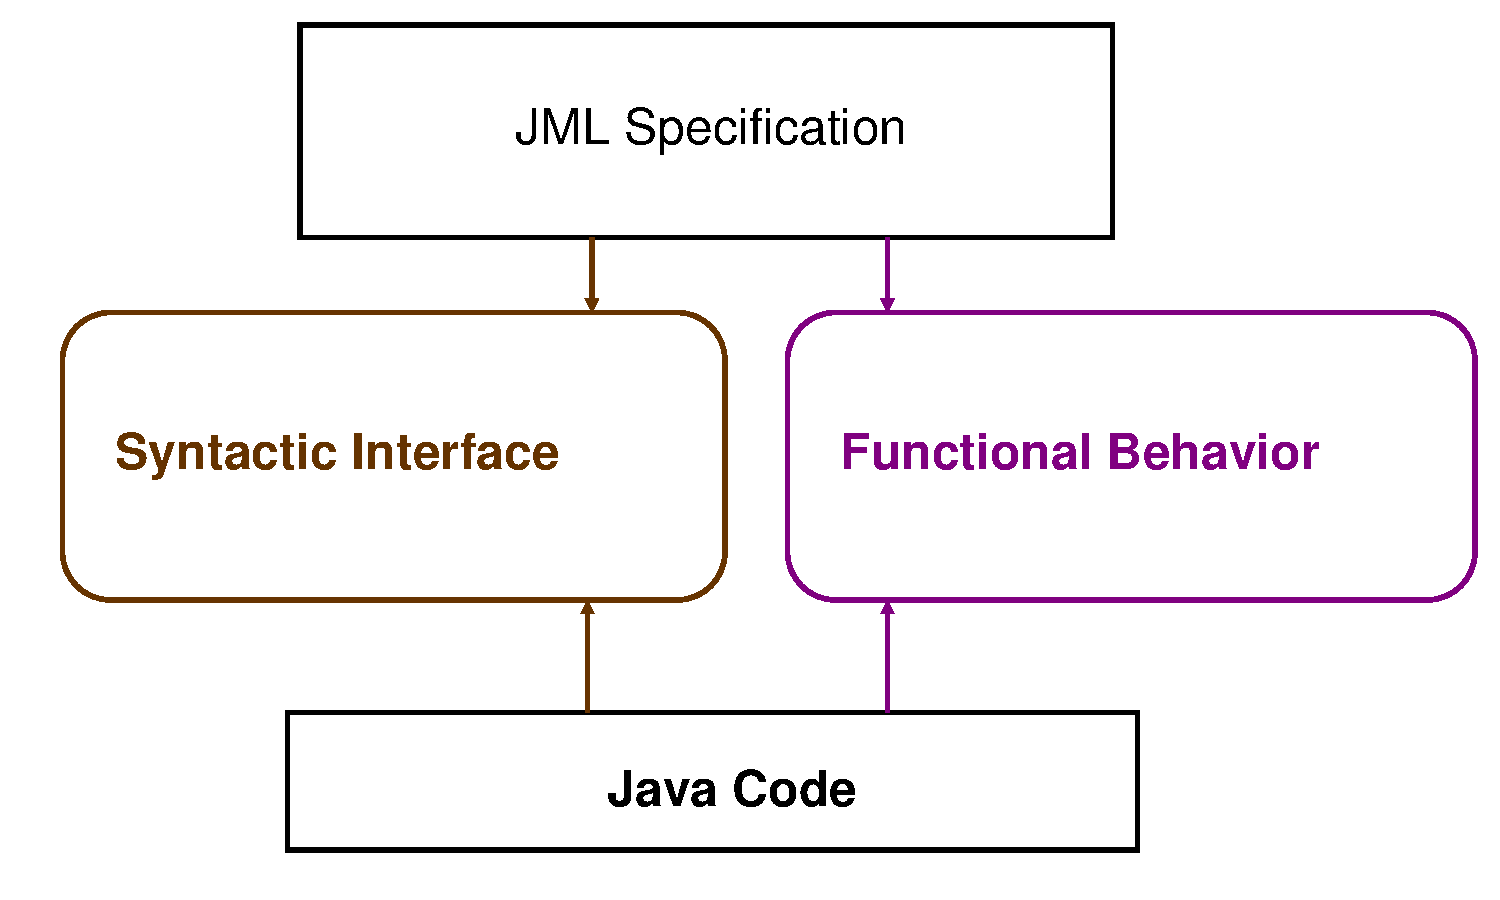
\includegraphics[width=4.25in]{if0}
\end{frame}

\begin{frame}
\frametitle{Interface Specification}
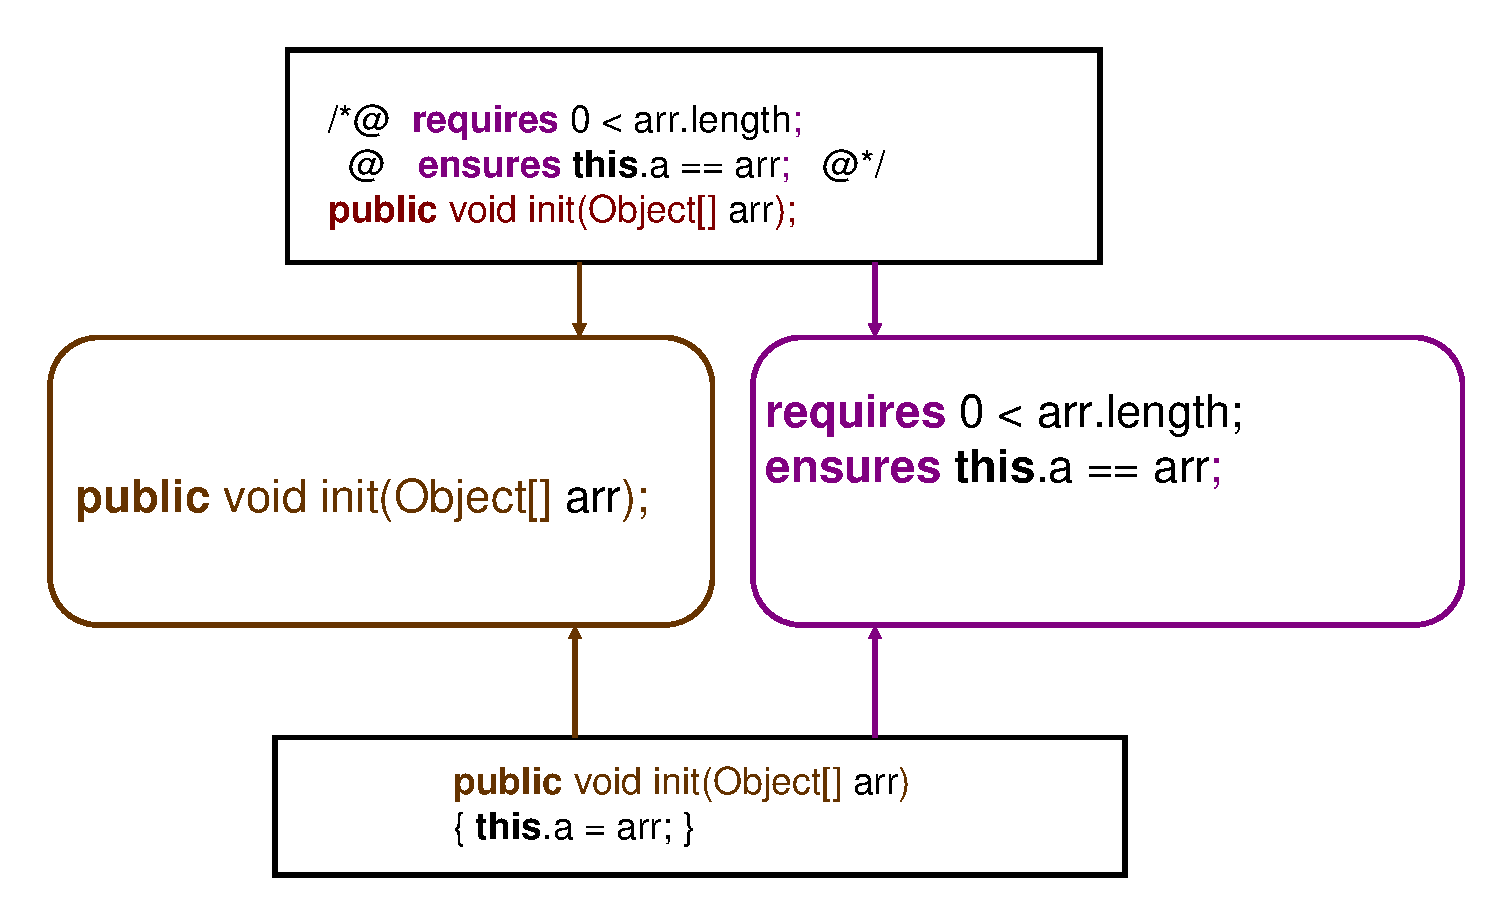
\includegraphics[width=4.25in]{if1}
\end{frame}

\begin{frame}
\frametitle{Like $\ldots$ But for Java and $\ldots$}
\begin{itemize}
\item
\textcolor{blue}{VDM}, but
\begin{itemize}
\item
OO features
\end{itemize}

\item
\textcolor{blue}{Eiffel}, but
\begin{itemize}
\item
Features for formal verification
\end{itemize}

\item
\textcolor{blue}{Spec\#}, but
\begin{itemize}
\item
Different invariant methodology
\item
More features for formal verification
\end{itemize}
\end{itemize}
\end{frame}

\begin{frame}
\frametitle{Unlike OCL and Z}

\begin{itemize}
\item
tailored to Java semantics.

\item
more Java-like syntax.
\end{itemize}

\end{frame}

\begin{frame}
\frametitle{Many Tools, One Language}
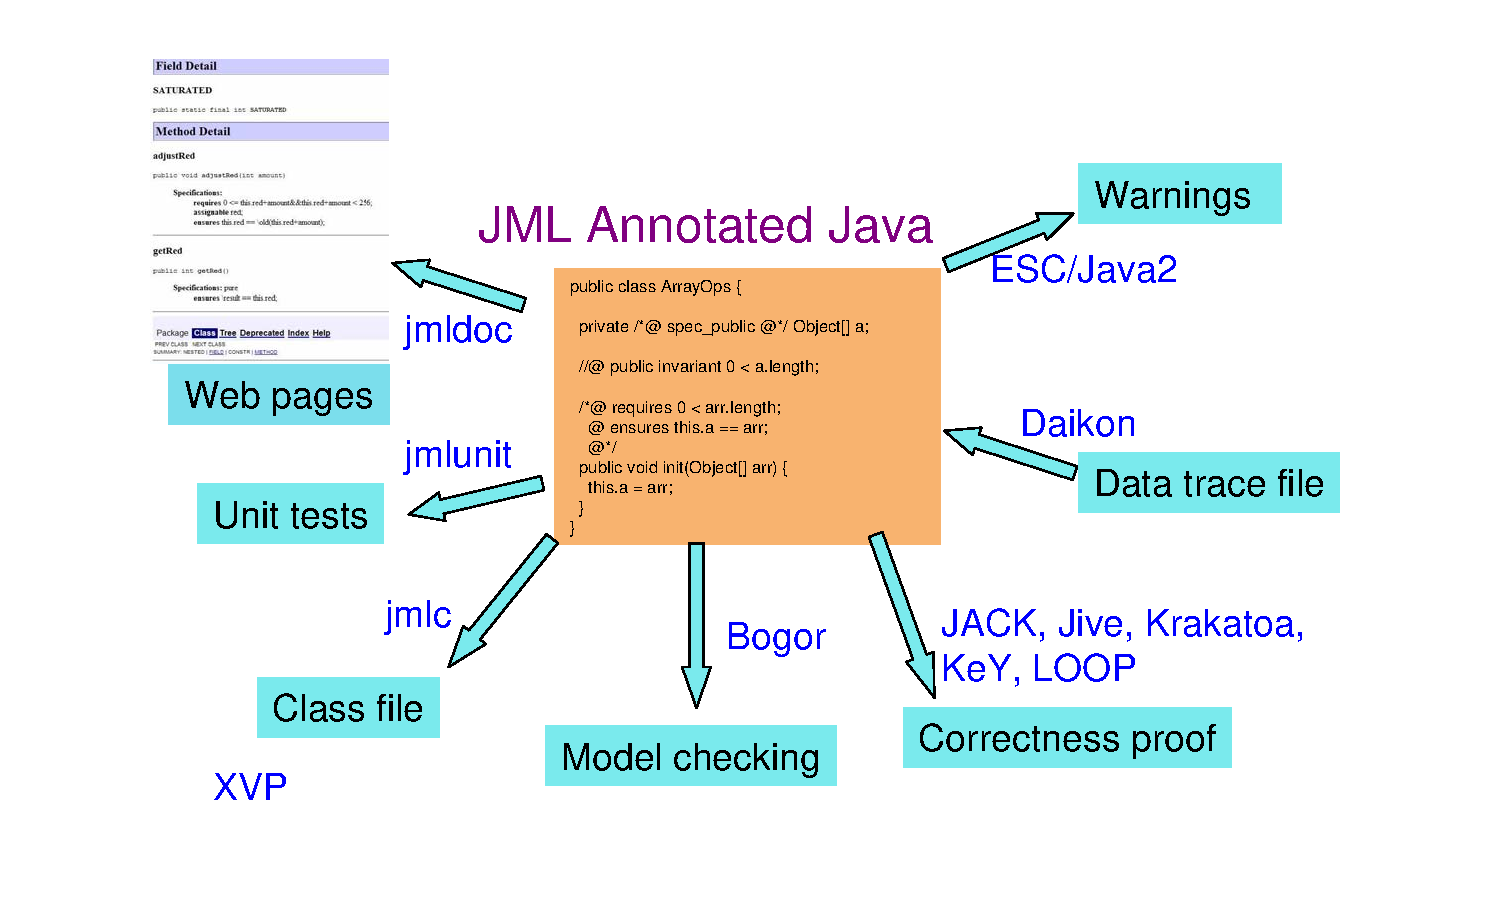
\includegraphics[width=4.25in]{tools-overview}
\end{frame}

\begin{frame}
\frametitle{How Tools Complement Each Other}
\begin{itemize}
\item
Different strengths:
\begin{itemize}
\item
Runtime checking --- real errors.

\item
Static checking --- better coverage.

\item
Verification --- guarantees.
\end{itemize}

\item
Usual ordering:
\begin{enumerate}
\item
Runtime checker (jmlc and jmlunit).

\item
Extended Static Checking (ESC/Java2).

\item
Verification tool (e.g., KeY, JACK, Jive).
\end{enumerate}
\end{itemize}
\end{frame}

\subsection[Importance]{Importance of JML}

\begin{frame}
\frametitle{Importance of JML}

\begin{itemize}
\item
Many tools.

\item
State of the art language.

\item
Large and open research community:
\begin{itemize}
\item
23 groups, worldwide.

\item
Over 135 papers.
\end{itemize}
\end{itemize}

See \href{http://www.jmlspecs.org}{jmlspecs.org}
\end{frame}

\begin{frame}
\frametitle{Advantages of Working with JML}

\begin{itemize}
\item
Reuse language design.

\item
Ease communication with researchers.

\item
Share customers.
\end{itemize}

Join us!
\end{frame}

\subsection[Finding More]{Where to Find More}

\begin{frame}
\frametitle{Where to Find More: \href{http://www.jmlspecs.org}{jmlspecs.org}}

Documents:
\begin{itemize}
\item
\href{ftp://ftp.cs.iastate.edu/pub/leavens/JML/jmldbc.pdf}{``Design by Contract with JML''}

\item
\href{http://dx.doi.org/10.1007/s10009-004-0167-4}{``An overview of JML tools and applications''}

\item
\href{http://doi.acm.org/10.1145/1127878.1127884}{``Preliminary Design of JML''}

\item
\href{http://www.jmlspecs.org/jmlrefman/jmlrefman_toc.html}{``JML Reference Manual''}
\end{itemize}

Also:
\begin{itemize}
\item
Examples, teaching material.

\item
Downloads, sourceforge project.

\item
Links to papers, etc.
\end{itemize}

\end{frame}

\section[Reading and Writing]{Reading and Writing JML Specifications}

\subsection[Lightweight]{Lightweight Specification of Functional Behavior}

\begin{frame}
\frametitle{Most Important JML Keywords}

Top-level in classes and interfaces:
\begin{itemize}
\item
\lstinline!invariant!

\item
\lstinline!spec_public!
\end{itemize}

For methods and constructors:
\begin{itemize}
\item
\lstinline!requires!

\item
\lstinline!ensures!

\item
\lstinline!assignable!

\item
\lstinline!pure!
\end{itemize}
\end{frame}

\begin{frame}
\frametitle{Example: BoundedStack}

\begin{example}
Specify bounded stacks of objects.
\end{example}

\note{See the file BoundedStack.java}
\end{frame}

\begin{frame}[fragile]
\frametitle{BoundedStack's Data and Invariant}
\lstinputlisting[linerange={1-12}]{examples/BoundedStack.java}
\note{Explain notation. Stress client view.}
\end{frame}

\begin{frame}[fragile]
\frametitle{BoundedStack's Constructor}
\lstinputlisting[linerange={13-19}]{examples/BoundedStack.java}
\end{frame}

\begin{frame}[fragile]
\frametitle{BoundeStack's push Method}
\lstinputlisting[linerange={21-32}]{examples/BoundedStack.java}
\end{frame}

\begin{frame}[fragile]
\frametitle{BoundeStack's pop Method}
\lstinputlisting[linerange={34-45}]{examples/BoundedStack.java}
\end{frame}

\begin{frame}[fragile]
\frametitle{BoundeStack's top Method}
\lstinputlisting[linerange={47-54}]{examples/BoundedStack.java}
\end{frame}

\begin{frame}[fragile]
\frametitle{spec\_public and invariant}

\lstinline!spec_public!
\begin{itemize}
\item
Public visibility.

\item
Only for specification purposes.
\end{itemize}

\note{\lstinline!spec_public! actually a syntactic sugar.}

\lstinline!invariant! must be:
\begin{itemize}
\item
True at end of constructor.

\item
Preserved by each method.
\end{itemize}

\note{Helper methods are an exception to invariant preservation.}
\end{frame}

\begin{frame}[fragile]
\frametitle{requires and ensures}

\lstinline!requires! clause:
\begin{itemize}
\item
Precondition.

\item
Obligation on callers, after parameter passing.

\item
Assumed by implementor.
\end{itemize}

\lstinline!ensures! clause:
\begin{itemize}
\item
Postcondition.

\item
Obligation on implementor, at return.

\item
Assumed by caller.
\end{itemize}
\end{frame}

\begin{frame}
\frametitle{Semantics of Requires and Ensures}
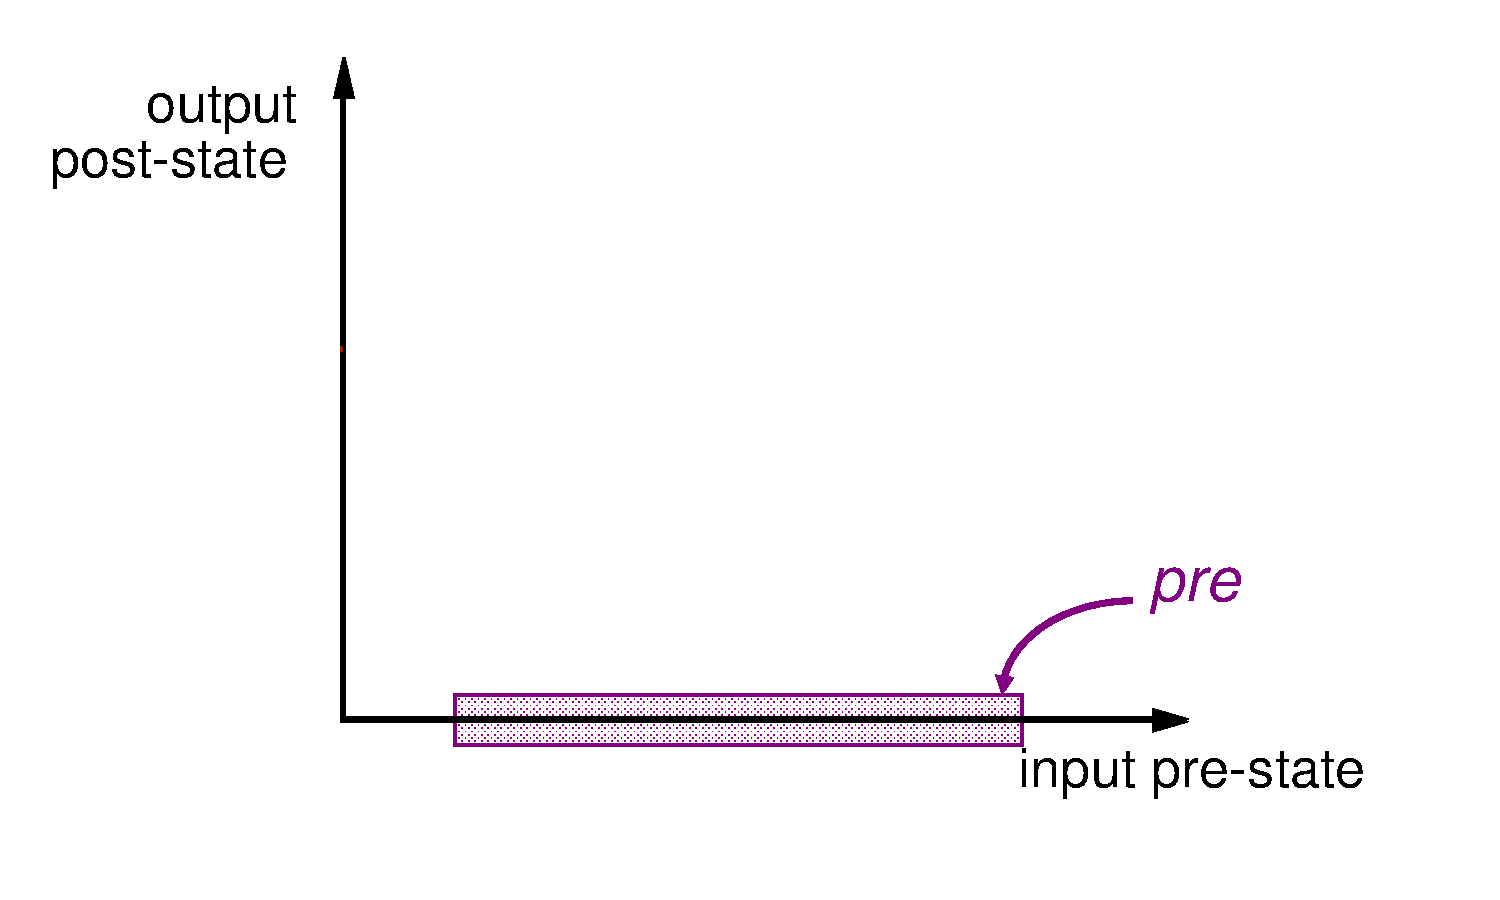
\includegraphics[width=4.25in]{requires}
\end{frame}

\begin{frame}
\frametitle{Semantics of Requires and Ensures}
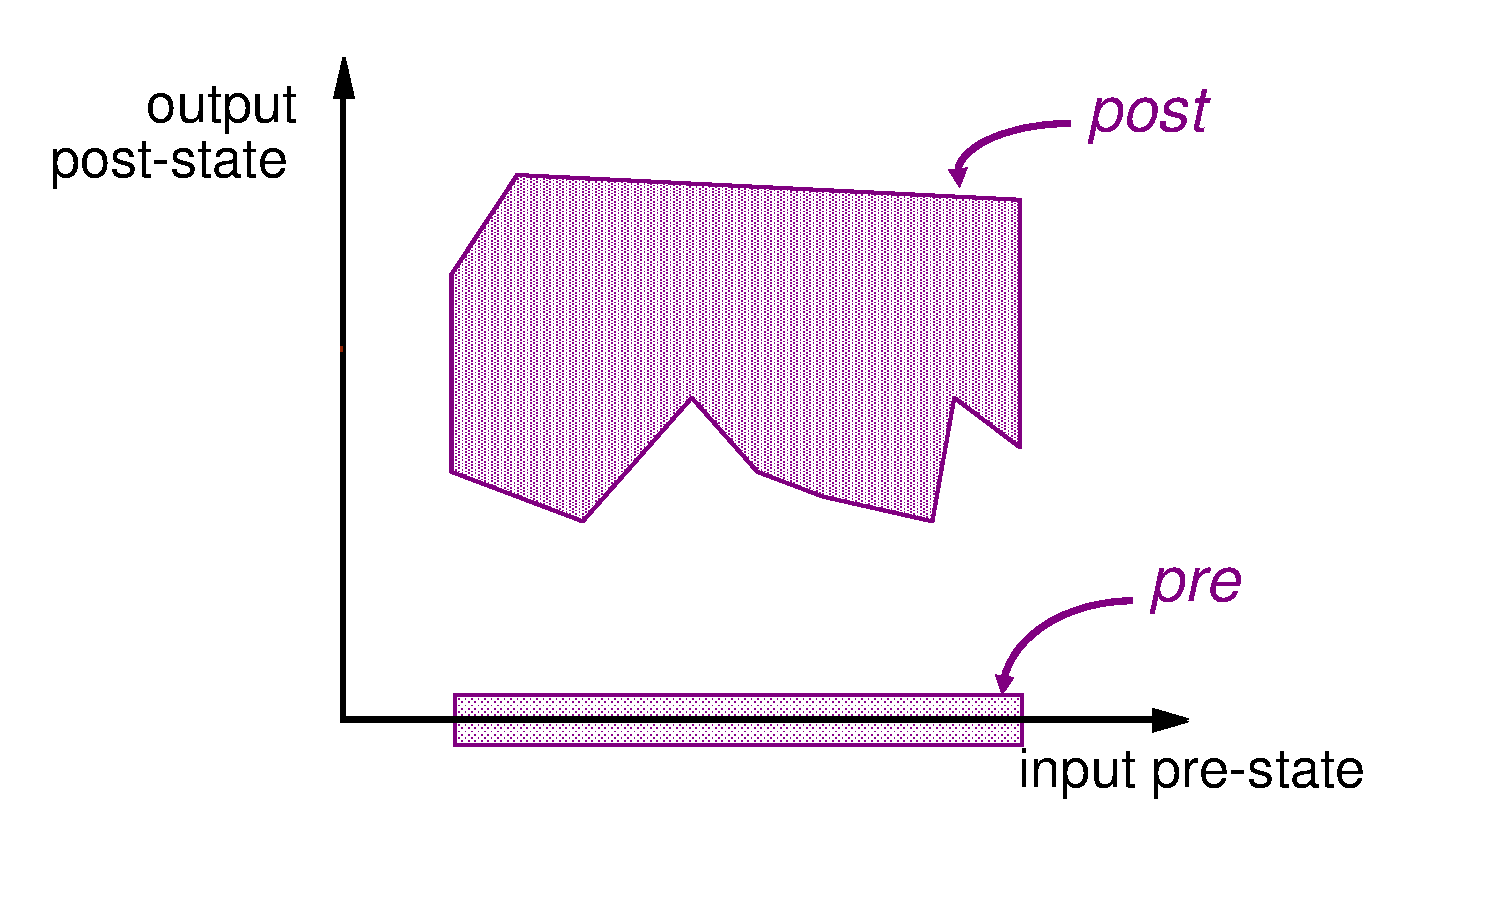
\includegraphics[width=4.25in]{ensures}
\end{frame}

\begin{frame}
\frametitle{Semantics of Requires and Ensures}
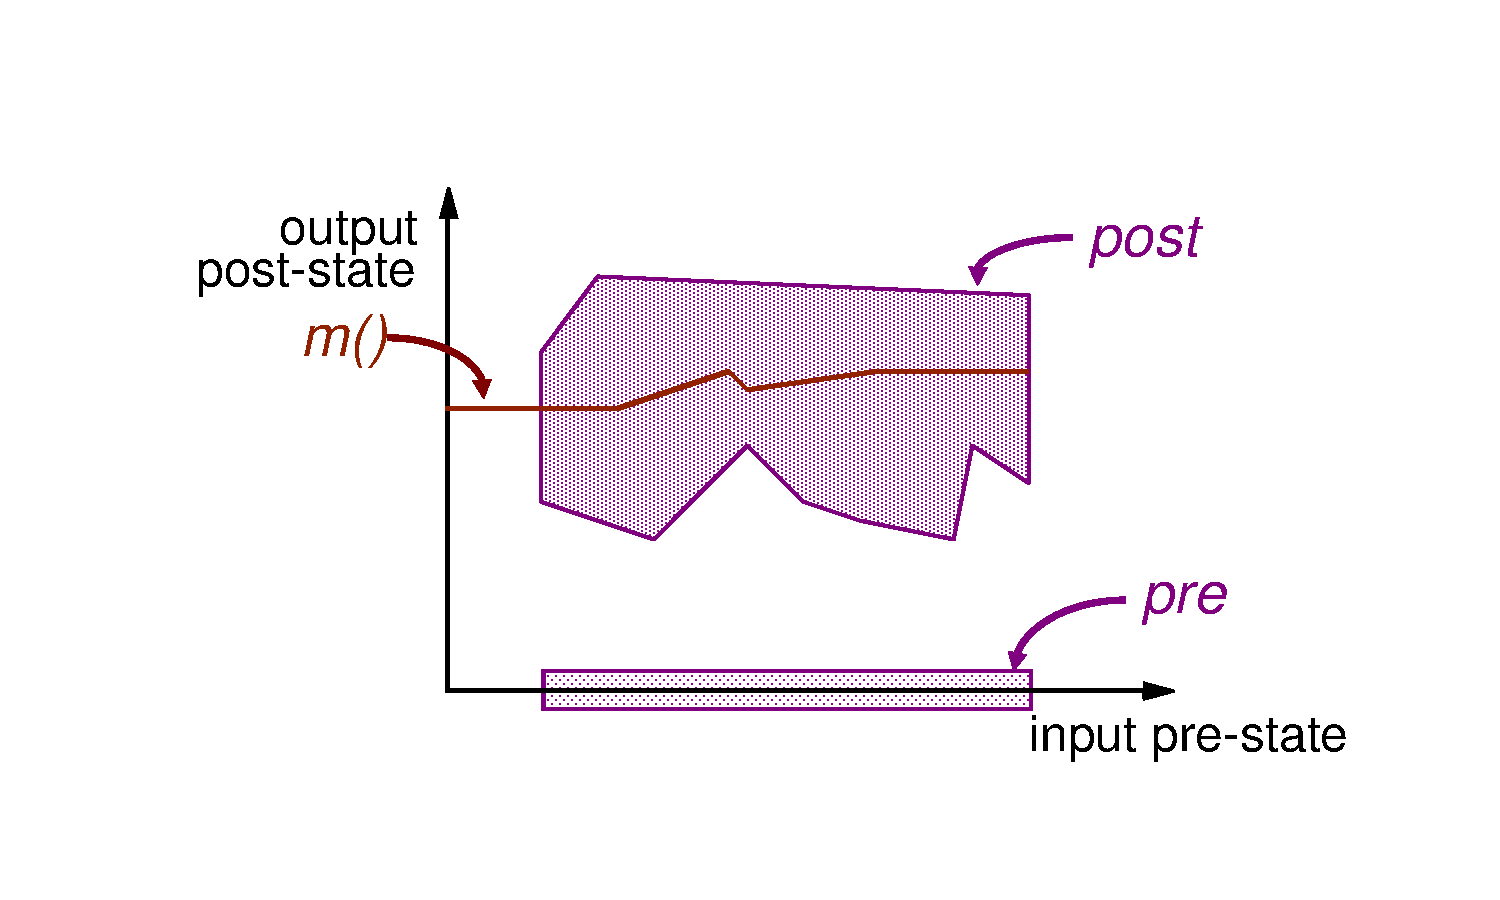
\includegraphics[width=4.25in]{correctimpl}
\end{frame}

\begin{frame}[fragile]
\frametitle{assignable and pure}

\lstinline!assignable!
\begin{itemize}
\item
Frame axiom.

\item
Locations (fields) in pre-state.

\item
New object fields not covered.

\item
Sugar for postcondition: ``nothing else assigned''

\item
Checked statically.

\item
Synonyms: \lstinline!modifies!, \lstinline!modifiable!
\end{itemize}

\lstinline!pure!
\begin{itemize}
\item
No side effects.

\item
Implies \lstinline!assignable \nothing!

\item
Allows method's use in specifications.
\end{itemize}
\end{frame}

\begin{frame}[fragile]
\frametitle{Redundant Clauses}

E.g., \lstinline!ensures_redundantly!
\begin{itemize}
\item
Alerts reader.

\item
States something to prove.

\item
Must be implied by:
\begin{itemize}
\item
\lstinline!ensures! clauses,

\item
\lstinline!assignable! clause,

\item
\lstinline!invariant!, and

\item
JML semantics.
\end{itemize}
\end{itemize}

Also \lstinline!requires_redundantly!, etc.
\end{frame}

\begin{frame}[fragile]
\frametitle{Multiple Clauses}

Semantics:

\begin{lstlisting}[mathescape=true]
  requires $P$;
  requires $Q$;
\end{lstlisting}

is equivalent to:

\begin{lstlisting}[mathescape=true]
  requires $P$ && $Q$;
\end{lstlisting}

Similarly for \lstinline!ensures!, \lstinline!invariant!.

~

Note: runtime checker gives better errors if separate.

\note{For assignable, semantics is the union.}
\end{frame}

\begin{frame}[fragile]
\frametitle{Expression Keywords}

\begin{itemize}
\item
\lstinline!\result! ~~ = ~~ method's return value.

\item
\lstinline[mathescape=true]!\old($E$)! ~~ = ~~ pre-state value of $E$.

\item
\lstinline[mathescape=true]!(\forall T x; $P$; $Q$)!
~~ = ~~ $\bigwedge \{ Q \mid x \in T \wedge P \}$

\item
\lstinline[mathescape=true]!(\exists T x; $P$; $Q$)!
~~ = ~~ $\bigvee \{ Q \mid x \in T \wedge P \}$

\item
\lstinline[mathescape=true]!(\min T x; $P$; $E$)!
~~ = ~~ $\min \{E \mid x \in T \wedge P \}$

\item
\lstinline[mathescape=true]!(\sum T x; $P$; $E$)!
~~ = ~~ $\sum \{E \mid x \in T \wedge P \}$

\item
\lstinline[mathescape=true]!(\num_of T x; $P$; $Q$)!
~~ = ~~ $\sum \{1 \mid x \in T \wedge P \wedge Q\}$

\item
$\ldots$
\end{itemize}
\end{frame}

\subsection[Exercise]{Specifying a Type}

\begin{frame}[fragile]
\frametitle{Steps for Specifying a Type}

\begin{enumerate}
\item
Specify data (\lstinline!spec_public! fields).

\item
Specify an \lstinline!invariant!.

\item
Specify each method with:

\begin{enumerate}
\item
\lstinline!requires!.

\item
\lstinline!ensures!.

\item
\lstinline!assignable! or \lstinline!pure!.
\end{enumerate}
\end{enumerate}
\end{frame}

\begin{frame}[fragile]
\frametitle{Exercise: Specify BagOfInt}

\begin{exercise}
Specify the following:

\rm
\lstinputlisting[language=Java,commentstyle=\itshape]{examples/BagOfInt.jml-refined}
\end{exercise}
\end{frame}

\begin{frame}<beamer>[fragile]
\frametitle{My Solution: BagOfInt's Data}

\lstinputlisting[language={[JML]Java},linerange={2-9}]{examples/BagOfInt.jml}
\note{Why do we need n?  To allow deletion.}
\end{frame}

\begin{frame}<beamer>[fragile]
\frametitle{My Solution: BagOfInt's Constructor}

\lstinputlisting[language={[JML]Java},linerange={11-16}]{examples/BagOfInt.jml}
\end{frame}

\begin{frame}<beamer>[fragile]
\frametitle{My Solution: Method occurrences}

\lstinputlisting[language={[JML]Java},linerange={18-23}]{examples/BagOfInt.jml}
\end{frame}

\begin{frame}<beamer>[fragile]
\frametitle{My Solution: Method extractMin}

\lstinputlisting[language={[JML]Java},linerange={25-33}]{examples/BagOfInt.jml}
\end{frame}


\subsection[Tool Use]{Basic Tool Use}  % demo + exercise

\subsection[Tips]{Tips and Pitfalls}

%\part{Advanced JML}

\section{Subtyping}

\section[Abstraction]{Abstraction in Specification}

\section[ESC]{ESC/Java2}

\section*{Conclusions}

%\appendix

\end{document}


% \begin{frame}
% \frametitle{What Are Prime Numbers?}
% \begin{definition}
% A \alert{prime number} is a number that has exactly two divisors.
% \end{definition}
% \begin{example}
% \begin{itemize}
% \item 2 is prime (two divisors: 1 and 2).
% \item 3 is prime (two divisors: 1 and 3).
% \item 4 is not prime (\alert{three} divisors: 1, 2, and 4).
% \end{itemize}
% \end{example}
% \end{frame}
